\chapter{Computational Experiments}\label{chp:computational-experiments}

\section{Multi-Agent-Based Simulation}\label{sec:multi-agent-based-simulation}

This section presents the results obtained from the \gls{mabs} described in
Section~\ref{sec:mabs-dengue-virus}. The implementation uses GAMA Platform
version 1.9.2, the OSMnx Python Library~\cite{boeing:2017} 1.9.3 was used to
extract the map from \gls{osm}, and the street blocks are computed using the
procedure described in Section~\ref{sec:city-block-labeling}. The code is
available in this public repository on
Github\footnote{\url{https://github.com/cvaraujo/dengue-cbrp-mabs}}.

This study explores different combinations of parameters from
Table~\ref{tab:initial-pop-params} to identify the optimal configuration for
each city based on the average number (min and max) of cases per week in
multiple simulation runs. The precision and reliability of the results are
assessed through the Pearson correlation coefficient ($r$), \gls{mae}, and the
analysis of the simulated endemic channel.

\begin{table}[ht!]
	\centering
	\caption{Parameters for the initial state of the simulation.}
	\label{tab:initial-pop-params}
	\resizebox{\textwidth}{!}{%
		\begin{tabular}{c|l|c}
			\toprule
			Parameter & Description                                                              & Value                  \\
			\midrule
			$p$       & Number of people per $m^2$                                               & 0.006 - 0.01           \\
			$H_b$     & Number of people in block b                                              & $p \times A_b$         \\
			$H_0$     & Starting size of human population                                        & $\sum_{b = 1}^{B} H_b$ \\
			$M_h$     & Number of mosquitoes per human                                           & 0.50 - 3.00            \\
			$M_b$     & Percent of infected mosquitoes in a block without notifications          & 0.05 - 0.30            \\
			$M_{b}^i$ & Percent of infected mosquitoes in a block with at least one notification & 0.40 - 0.90            \\
			$BS$      & Number of potential Breeding Sites                                       & 50 - 500               \\
			\bottomrule
		\end{tabular}%
	}
\end{table}

\subsection{Data Processing}\label{subsec:data-processing}

First, the objective is to establish the initial population size by computing
the $p$ values. This work calculates the area of each street block as a polygon
using the Shapely\footnote{\url{https://shapely.readthedocs.io/en/stable/}} and
Geopandas\footnote{\url{https://geopandas.org/en/stable/}} Python libraries with
data imported from \gls{osm}. Since the investigation in this work focuses
mainly on urban areas, and both cities have vast territorial extensions that are
predominantly composed of rural areas, their overall population densities
reported in \gls{ibge} are low. For this reason, this work restricts the area
considered in the population density calculation to the city center and strictly
adjacent zones. However, there are no population data available at the level of
blocks or neighborhoods, and alternative sources were needed to improve the
values that estimate the resident population in the cities and then define the
initial population parameters for the simulation.

The choice of using a parameter ($p$) defined as persons per square meter
(m\textsuperscript{2}) ensures a good level of generalization for the
simulation, as the presence of this value allows the population to remain
proportionally adjusted for different experiments changing the size of the city
map. This can be particularly useful, for example, if we wish to simulate the
evolution of dengue cases in a single neighborhood.

Based on data provided by \gls{osm}, the urban area considered in Alto Santo
covers approximately 0.9~km\textsuperscript{2}, with an estimated population of
9,000 people living in the city centers. This yields a population density of $p
	= 0.01$ people per m\textsuperscript{2}. For Limoeiro, the approximate urban
area has 6~km\textsuperscript{2} and a population of 36000, which corresponds to
a value of \( p = 0.006 \) people per m\textsuperscript{2}. Since this
\gls{mabs} positions the individuals within blocks, the starting human
population consists of the sum of $p$ multiplied by the area of the
corresponding block. For Alto Santo, using a radius of 700~m inside OSMnx, 73
street blocks are generated and the starting human population is $H_0 = 5688$.
In Limoeiro, with a large urban area, the radius of 2000~m provides 563 blocks
and an initial population $H_0 = 29914$.

The starting size of the mosquito population is determined by $m = H_b \times
	M_h$, where the number of infected mosquitoes in the block is $M_b \times m$ for
blocks without cases and $M_b^{i} \times m$ otherwise. The starting number of
potential breeding sites is related to the parameter $BS$ and the blocks. For
each block, if there is at least one positive case, then there is at least one
breeding site. At the end of the initial scenario creation, if the breeding
sites located are fewer than $BS$, then the remaining were placed in random
blocks.

The \gls{mabs} initialize using epidemiological data from a specified start
date, incorporating historical notifications from the preceding week as
confirmed cases within the simulation blocks. This methodology is in line with
standard public health surveillance practices. To validate accuracy and quality,
the simulated case projections are systematically compared with actual weekly
reported cases over a 90-day evaluation period (equivalent to 180 simulation
cycles after initialization). The selected starting dates are selected based on
epidemiological periods within a reasonable number of notifications, as explored
in Section~\ref{sec:real-notifications}.

The parameters tested were $M_h = [0.5, 1, 2, 3]$, $M_b = [0.05, 0.1, 0.15, 0.2,
	0.3]$, $M_b^{i} = [0.4, 0.5, 0.6, 0.7, 0.8]$, and $BS = [50, 100, 200, 300,
	500]$. The analysis aggregates the results of 100 independent simulation trials
for each parameter configuration and start date, ensuring statistical robustness
in assessing model performance. The default maps of Alto Santo and Limoeiro
consider OSMnx radius of 700~m and 2000~m, respectively.

An independent set of initial dates was defined for each city. The objective of
the parameter exploration is to determine the best configuration based on
similarity with historical real-world data, which were mapped to the same map
segment used in the simulation. One set of parameters is considered better than
another using the number of ``wins'' for the dates on which these three
criteria, in the following order of precedence, were better: (1) higher
correlation between the simulated mean and the real data; (2) lower \gls{mae}
between the simulated mean and the historical data; (3) number of weeks in which
the real case notifications fall within the Simulation Endemic Channel, i.e.,
the range between the highest and lowest number of simulated cases in a given
week. The concept of endemic channel is used by public health departments to
assess how the number of cases in the current \gls{ew} compares with the
historical in previous years.


\subsection{Results for Alto Santo}

To determine the start dates for the experiments, we selected the two years with
the highest number of positive or pending notifications (2017 and 2021). The
cases were then grouped by epidemiological week, as shown in
Figure~\ref{fig:cases-per-week-as}. The objective is to focus on periods with
the highest number of cases and consistency between adjacent weeks, while
avoiding intervals with few or no cases. The experiments explore different
starting dates within these periods to analyze the simulation's behavior when
initiated at distinct moments along the endemic curve. Only historical
notifications that can be assigned to a block in the simulation are considered,
ensuring a fair comparison.

For better visualization of the results achieved by the simulator,
Figure~\ref{fig:avg-result-2017-01-as} presents the results for the best
configuration considering the following starting dates: \textit{(1)}~2017-01-08,
\textit{(2)}~2017-01-15, \textit{(3)}~2017-01-22, \textit{(4)}~2017-01-29,
\textit{(5)}~2021-05-30, and \textit{(6)}~2021-06-06. The X-axis represents the
week number, the Y-axis represents the number of cases, the solid black line
represents the total real notifications in the week, the dashed line represents
the average number of cases across simulations with the same starting scenario,
and the light gray ``$\times$'' markers represent the number of cases for a
given simulation run.

\begin{figure}[!ht]
	\begin{minipage}[c]{.45\textwidth}
		\centering
		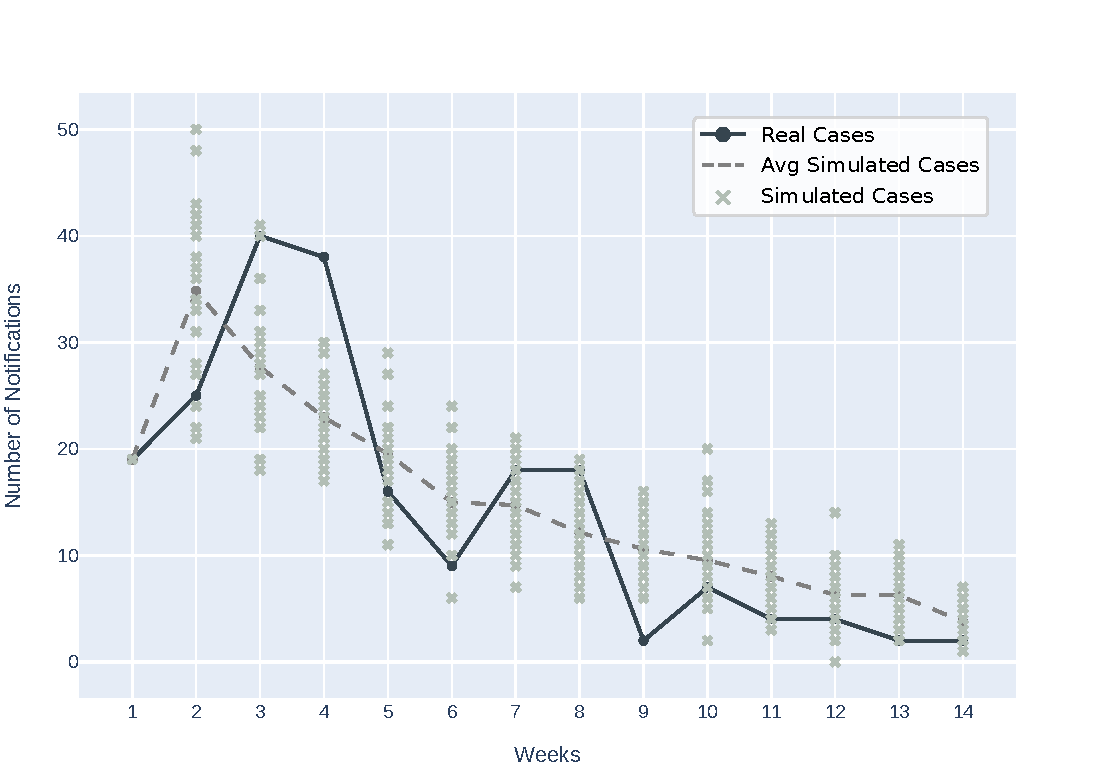
\includegraphics[scale=0.4]{images/experiments-as/AS-2017-01-08.pdf}
		\subcaption{\label{subfig:as-a} 2017-01-08}
	\end{minipage}
	\hspace{0.5cm}
	\begin{minipage}[c]{.45\textwidth}
		\centering
		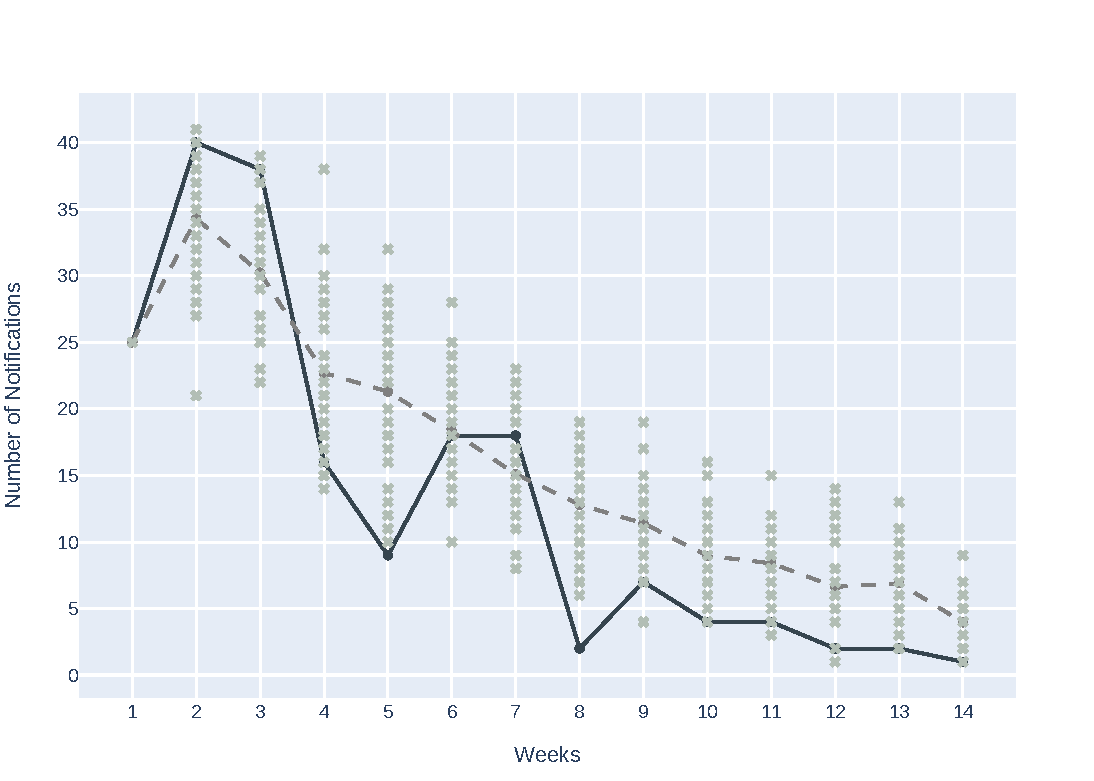
\includegraphics[scale=0.4]{images/experiments-as/AS-2017-01-15.pdf}
		\subcaption{\label{subfig:as-b} 2017-01-15}
	\end{minipage}
	\\
	\begin{minipage}[c]{.45\textwidth}
		\centering
		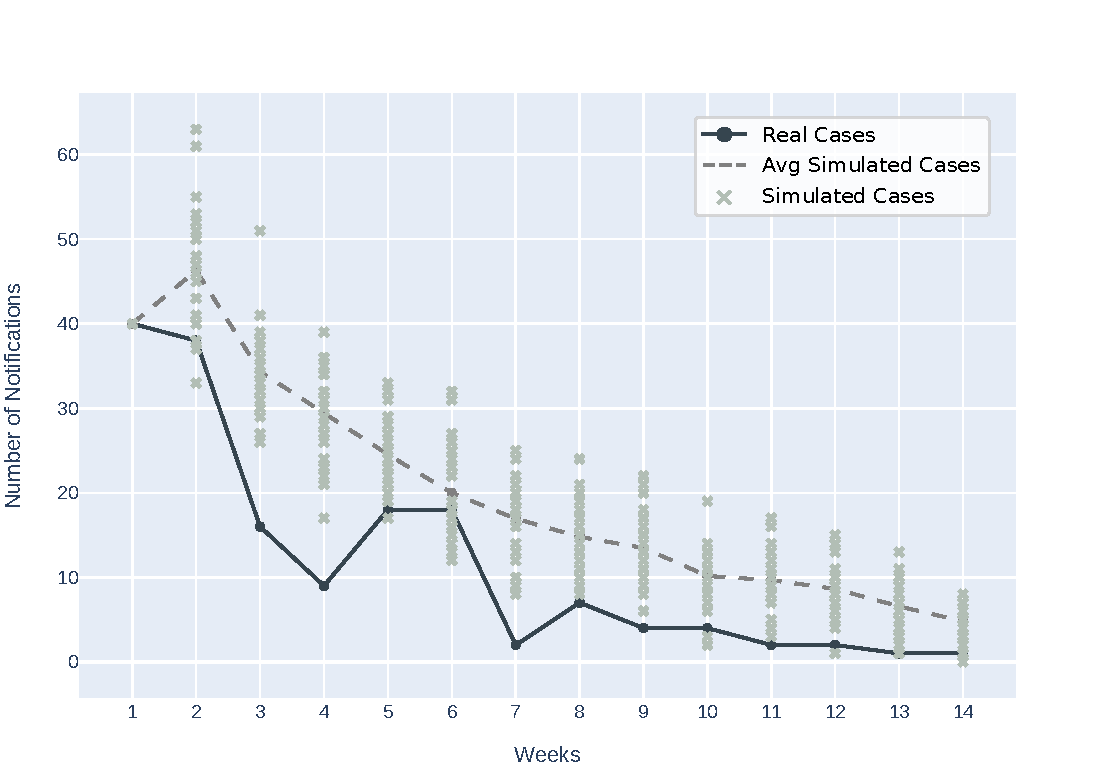
\includegraphics[scale=0.4]{images/experiments-as/AS-2017-01-22.pdf}
		\subcaption{\label{subfig:as-c} 2017-01-22}
	\end{minipage}
	\hspace{0.5cm}
	\begin{minipage}[c]{.45\textwidth}
		\centering
		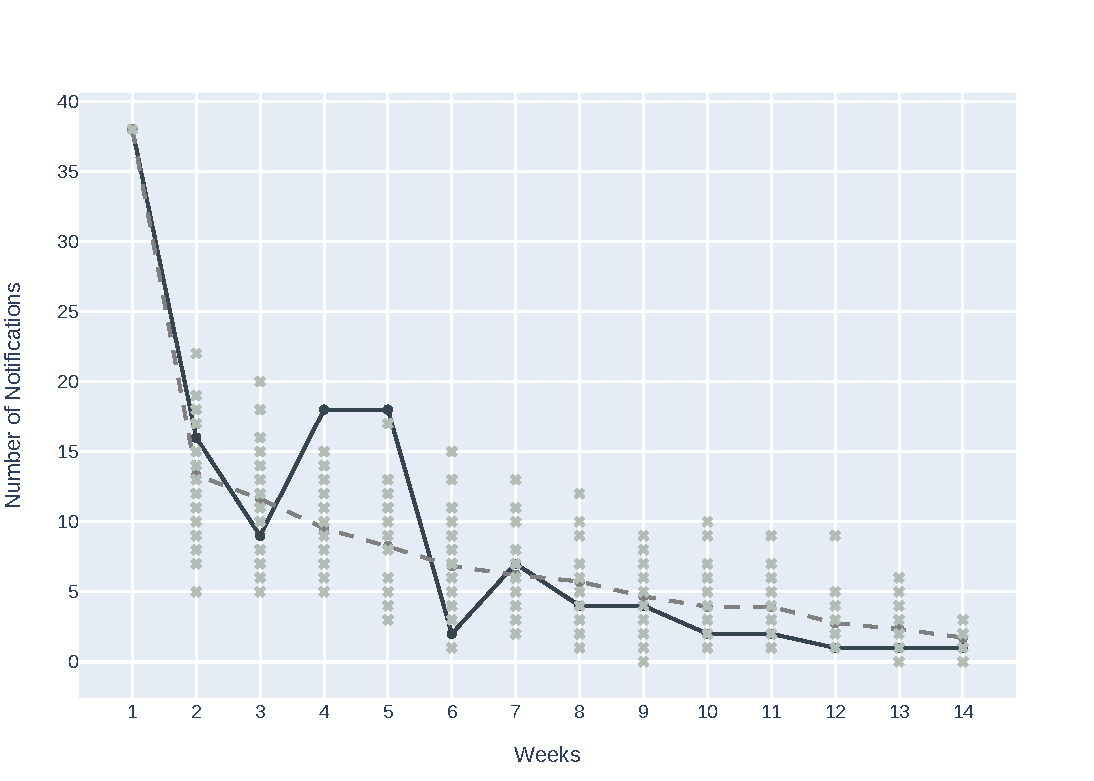
\includegraphics[scale=0.4]{images/experiments-as/AS-2017-01-29.pdf}
		\subcaption{\label{subfig:as-d} 2017-01-29}
	\end{minipage}
	\\
	\begin{minipage}[c]{.45\textwidth}
		\centering
		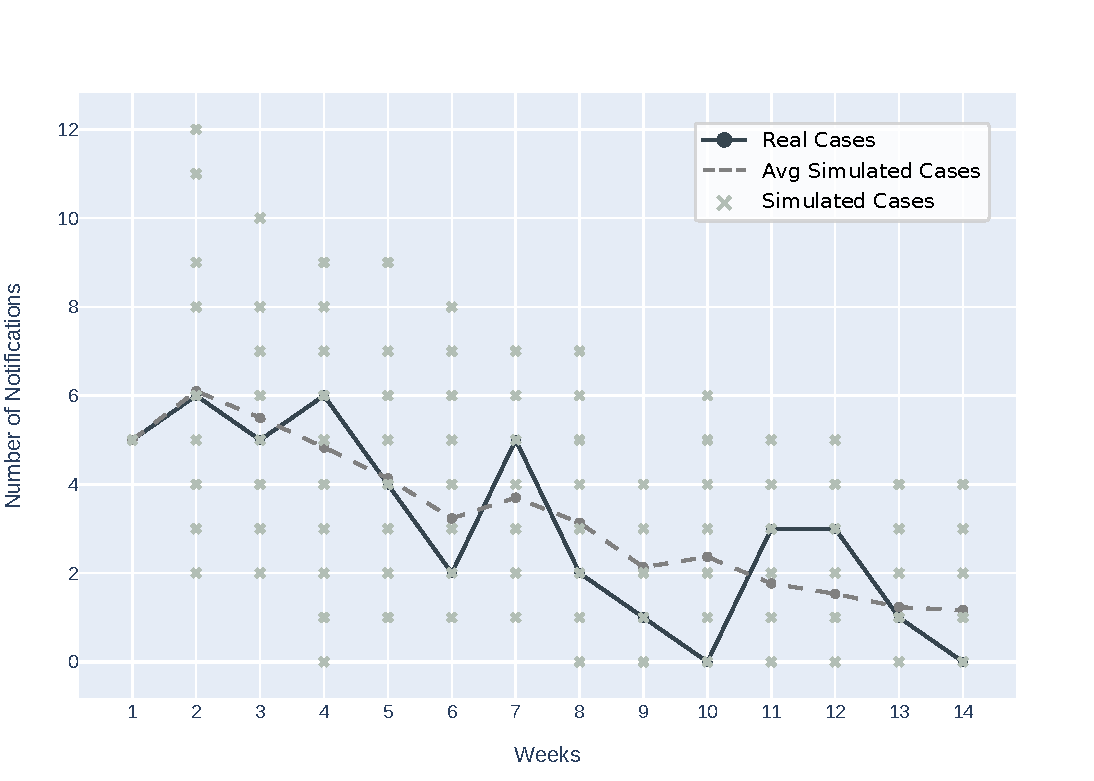
\includegraphics[scale=0.4]{images/experiments-as/AS-2021-05-30.pdf}
		\subcaption{\label{subfig:as-e} 2021-05-30}
	\end{minipage}
	\hspace{0.5cm}
	\begin{minipage}[c]{.45\textwidth}
		\centering
		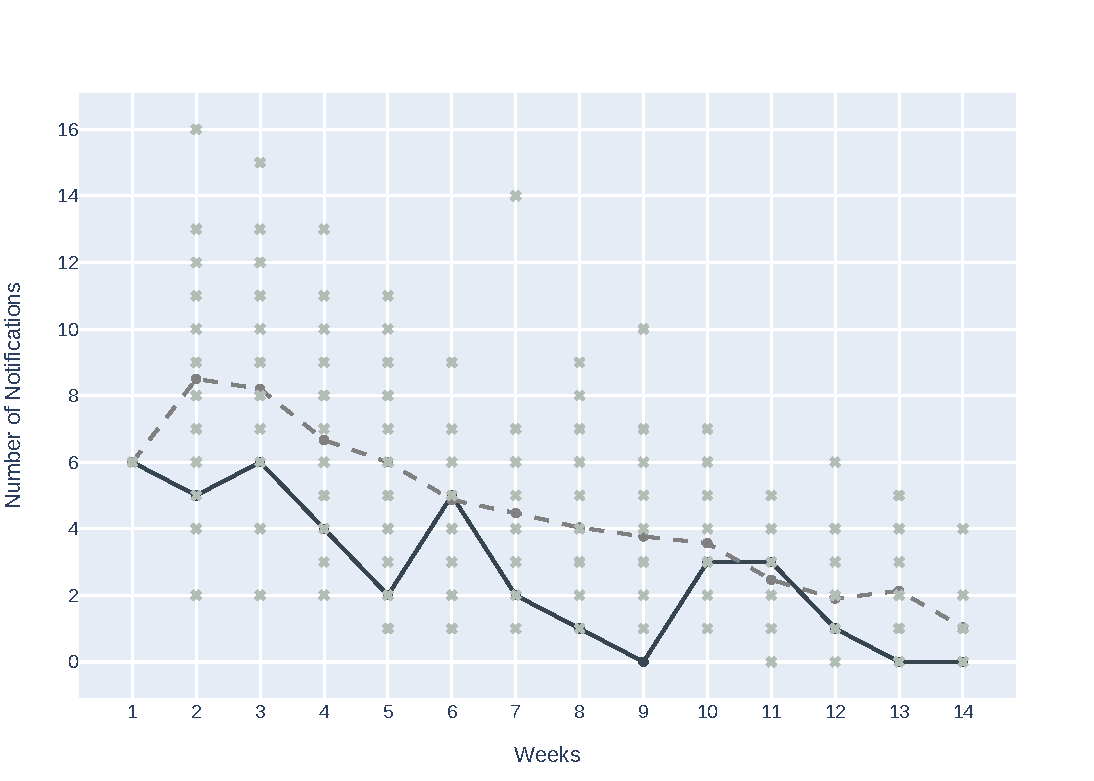
\includegraphics[scale=0.4]{images/experiments-as/AS-2021-06-06.pdf}
		\subcaption{\label{subfig:as-f} 2021-06-06}
	\end{minipage}
	\caption{\label{fig:avg-result-2017-01-as} Comparison of simulation and real cases from \textit{Alto Santo} for different starting dates.}
\end{figure}

The results represented in Figure~\ref{fig:avg-result-2017-01-as} correspond to
the variable parameters $M_h = 1$, $BS = 50$, $M_b = 0.05$ and $M_b^{i} = 0.4$,
which is the combination that achieved the best results considering the highest
correlation values ($r$) among all configurations for \textit{Alto Santo}. More
detailed information on these results is discussed later in this section.
%
Table~\ref{tab:statistical-data-as} shows the values of \gls{mae}, the
correlation of the average simulated cases with the real notification ($r$) and
the confidence interval (CI), in addition to the graphical results presented in
Figure~\ref{fig:avg-result-2017-01-as}.

\begin{table}[!ht]
	\centering
	\caption{Statistical values from the best configuration - \textit{Alto Santo} city.}
	\label{tab:statistical-data-as}
	\small{%
		\begin{tabular}{lrrrr}
			\toprule
			\multicolumn{1}{c}{\textbf{Date}}       &
			\multicolumn{1}{c}{\textbf{MAE}}        &
			\multicolumn{1}{c}{\textbf{$r$}}        &
			\multicolumn{1}{c}{\textbf{$CI_{min}$}} &
			\multicolumn{1}{c}{\textbf{$CI_{max}$}}                                      \\ \midrule
			2017-01-08                              & 5.67 & \textbf{0.83} & 0.61 & 0.94 \\
			2017-01-15                              & 5.20 & \textbf{0.93} & 0.82 & 0.97 \\
			2017-01-22                              & 8.40 & \textbf{0.90} & 0.75 & 0.96 \\
			2017-01-29                              & 2.80 & \textbf{0.92} & 0.80 & 0.97 \\
			2021-05-30                              & 0.94 & \textbf{0.84} & 0.62 & 0.94 \\
			2021-06-06                              & 1.92 & \textbf{0.77} & 0.49 & 0.91 \\ \bottomrule
		\end{tabular}%
	}
\end{table}

All experiments strongly correlate with real cases, achieving correlation
coefficients of at least $0.77$ with positive confidence intervals. This strong
correlation indicates that the average number of simulated cases per week
closely matches the real number of cases. The endemic channel generated in each
image of~\ref{fig:avg-result-2017-01-as} has a difference of at most 10 cases
from the real notifications when they are outside the endemic channel for a
given \gls{ew}, which represents a small deviation from reality.

\subsection{Results for Limoeiro}

The years 2019 and 2020 are selected for \textit{Limoeiro} city, and the number
of cases per week is shown in Figure~\ref{fig:cases-per-week-limoeiro}.
Figure~\ref{fig:avg-result-lim} presents the results for the following starting
dates: \textit{(1)}~2019-04-14, \textit{(2)}~2019-05-05,
\textit{(3)}~2020-06-21, \textit{(4)}~2020-07-05, \textit{(5)}~2020-07-19, and
\textit{(6)}~2020-07-26. Due to the extreme difference in the number of cases
between the two years for \textit{Limoeiro}, where 2020 has more than 1000
notifications than 2019, it was not possible to define a set of parameters that
fit well for both years with such different samples and behavior.
Figures~\ref{subfig:lim-a} and~\ref{subfig:lim-b} show the best results obtained
with the parameters $M_h = 0.5$, $BS = 100$, $M_b = 0.05$ and $M_b^{i} = 0.4$.
Figures~\ref{subfig:lim-c} to~\ref{subfig:lim-f} present the results with the
following parameters set $M_h = 1$, $BS = 500$, $M_b = 0.20$ and $M_b^{i} =
	0.9$.

\begin{figure}[!ht]
	\begin{minipage}[c]{.45\textwidth}
		\centering
		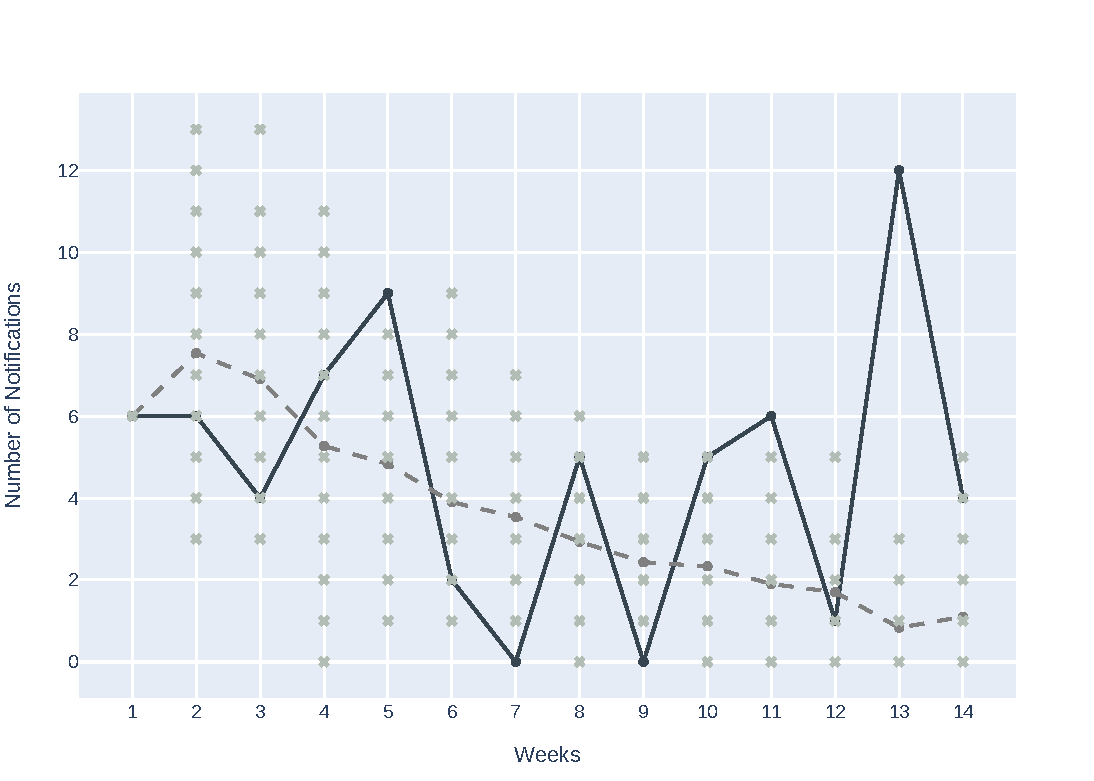
\includegraphics[scale=0.4]{images/experiments-lim/LIM-2019-04-14.pdf} \\
		\vspace{-0.3cm}
		\subcaption{\label{subfig:lim-a} 2019-04-14}
		% {\label{subfig:lim-a} 2019-04-14}
	\end{minipage}
	\hspace{0.5cm}
	\begin{minipage}[c]{.45\textwidth}
		\centering
		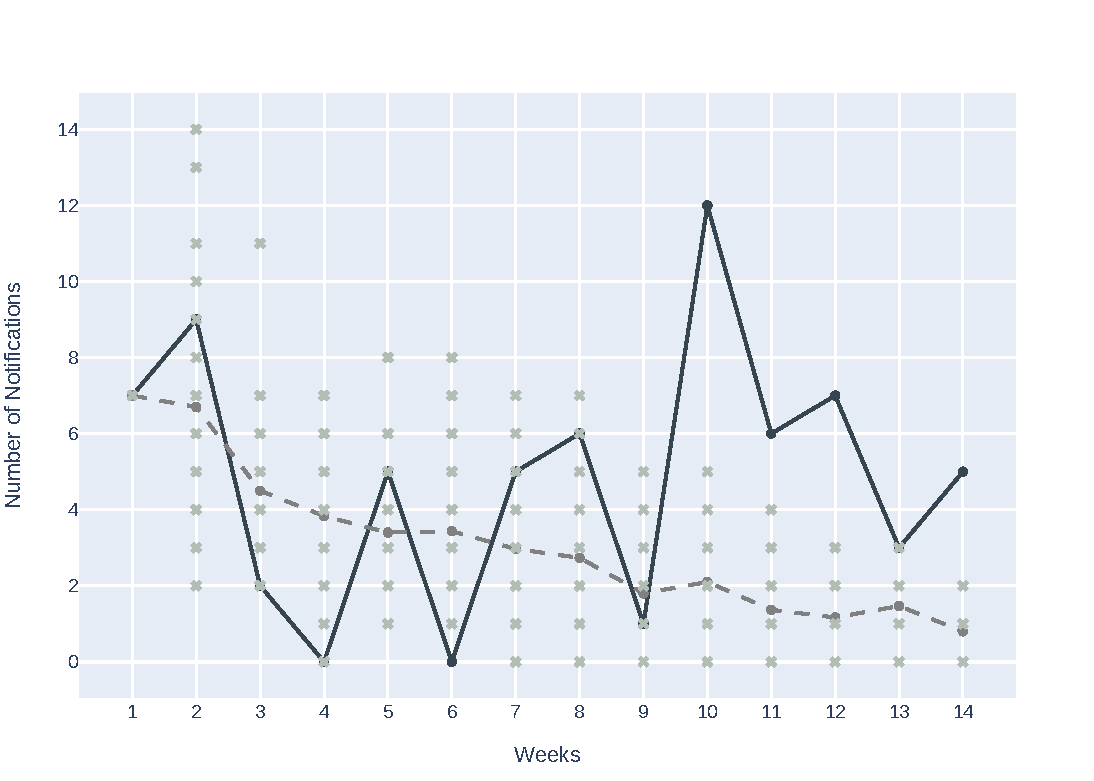
\includegraphics[scale=0.4]{images/experiments-lim/LIM-2019-05-05.pdf} \\
		\vspace{-0.3cm}
		\subcaption{\label{subfig:lim-b} 2019-05-05}
		% {\label{subfig:lim-b}\scriptsize (b) From 2019-05-05}
	\end{minipage}
	\\
	\begin{minipage}[c]{.45\textwidth}
		\centering
		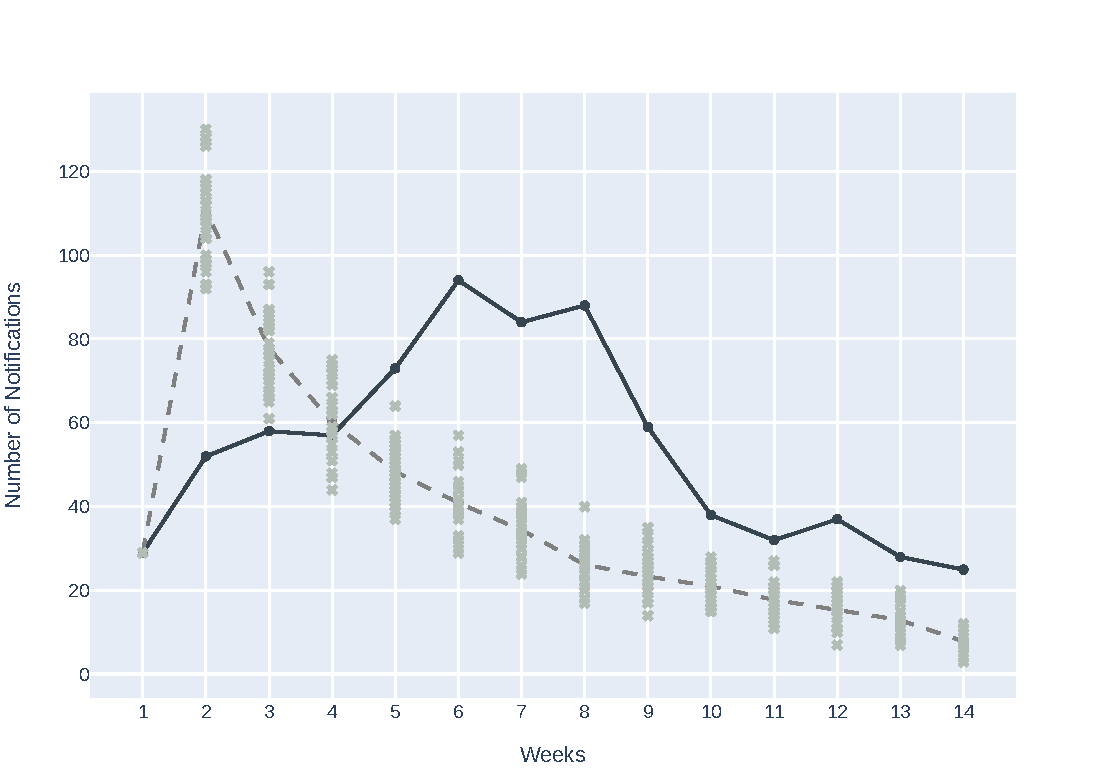
\includegraphics[scale=0.4]{images/experiments-lim/LIM-2020-06-21.pdf} \\
		\vspace{-0.3cm}
		\subcaption{\label{subfig:lim-c} 2020-06-21}
		% {\label{subfig:lim-c}\scriptsize (c) From 2020-06-21}
	\end{minipage}
	\hspace{0.5cm}
	\begin{minipage}[c]{.45\textwidth}
		\centering
		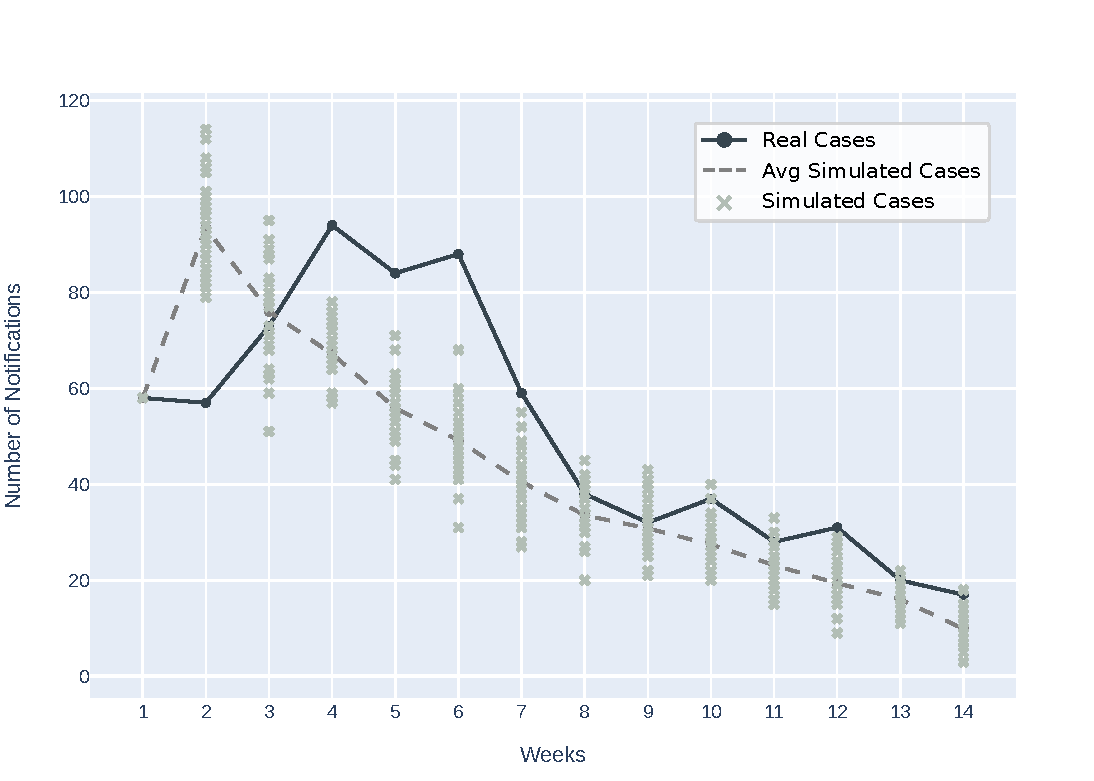
\includegraphics[scale=0.4]{images/experiments-lim/LIM-2020-07-05.pdf} \\
		\vspace{-0.3cm}
		\subcaption{\label{subfig:lim-d} 2020-07-05}
		% {\label{subfig:lim-d}\scriptsize (d) From 2020-07-05}
	\end{minipage}
	\\
	\begin{minipage}[c]{.45\textwidth}
		\centering
		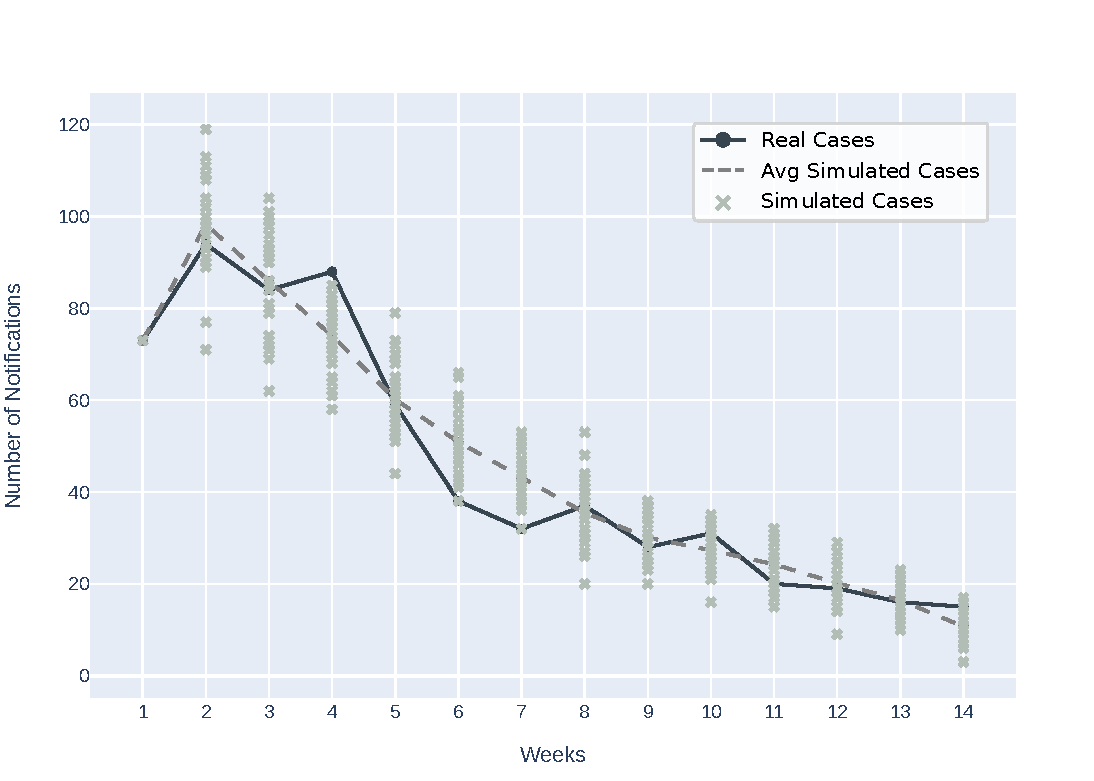
\includegraphics[scale=0.4]{images/experiments-lim/LIM-2020-07-19.pdf} \\
		\vspace{-0.3cm}
		\subcaption{\label{subfig:lim-e} 2020-07-19}
		% {\label{subfig:lim-e} \scriptsize (e) From 2020-07-19}
	\end{minipage}
	\hspace{0.5cm}
	\begin{minipage}[c]{.45\textwidth}
		\centering
		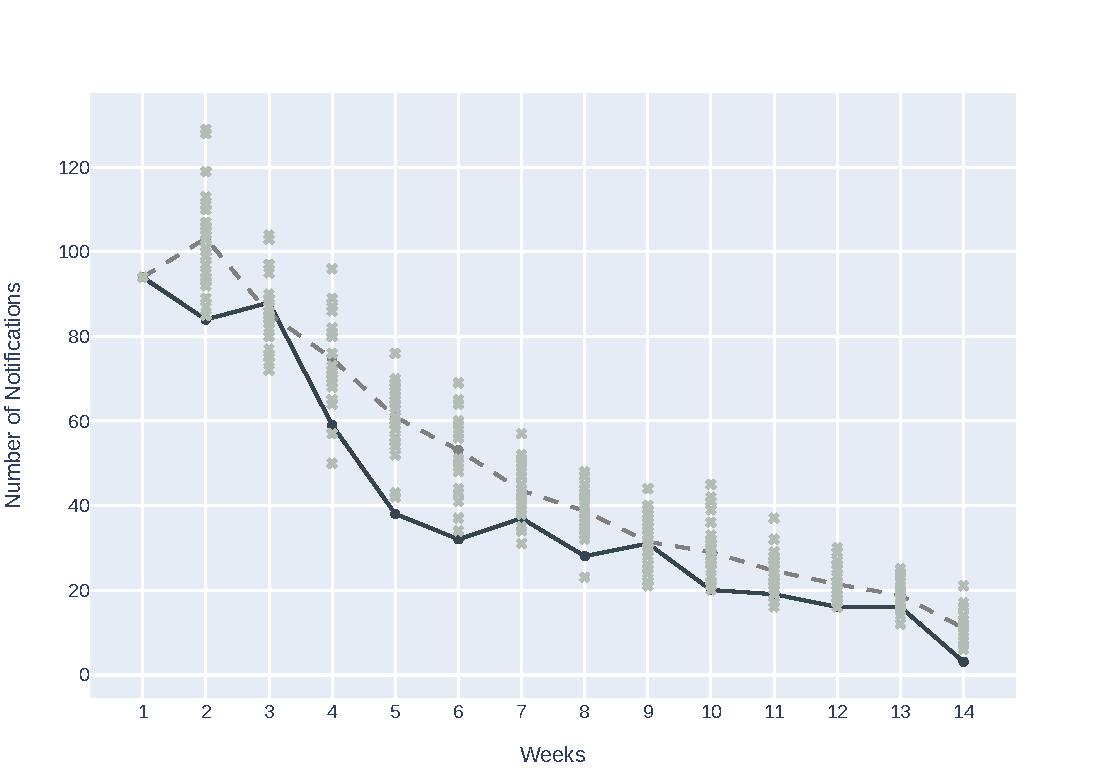
\includegraphics[scale=0.4]{images/experiments-lim/LIM-2020-07-26.pdf} \\
		\vspace{-0.3cm}
		\subcaption{\label{subfig:lim-f} 2020-07-26}
		% {\label{subfig:lim-f}\scriptsize (f) From 2020-07-26}
	\end{minipage}
	\caption{\label{fig:avg-result-lim} Comparison of simulation and real cases from \textit{Limoeiro} for different starting dates.}
\end{figure}

Table~\ref{tab:statistical-data-lim} shows the values of \gls{mae}, the correlation of the average simulated cases with the real notification ($r$), and the confidence interval of the results presented in Figures~\ref{fig:avg-result-lim}.

\begin{table}[!ht]
	\centering
	\caption{Statistical values from the best configuration - \textit{Limoeiro} city.}
	\label{tab:statistical-data-lim}
	\small{%
		\begin{tabular}{lrrrr}
			\toprule
			\multicolumn{1}{c}{\textbf{Date}}       &
			\multicolumn{1}{c}{\textbf{MAE}}        &
			\multicolumn{1}{c}{\textbf{$r$}}        &
			\multicolumn{1}{c}{\textbf{$CI_{min}$}} &
			\multicolumn{1}{c}{\textbf{$CI_{max}$}}                                        \\ \midrule
			2019-04-14                              & 2.99  & 0.06          & -0.41 & 0.51 \\
			2019-05-05                              & 3.28  & 0.09          & -0.38 & 0.53 \\
			2020-06-21                              & 27.97 & 0.30          & -0.18 & 0.67 \\
			2020-07-05                              & 13.90 & \textbf{0.76} & 0.45  & 0.90 \\
			2020-07-19                              & 4.49  & \textbf{0.97} & 0.93  & 0.99 \\
			2020-07-26                              & 9.27  & \textbf{0.96} & 0.90  & 0.99 \\ \bottomrule
		\end{tabular}%
	}
\end{table}

In 2019, the analysis of \textit{Limoeiro} City’s epidemiological data revealed
a weak correlation (values approaching zero), as indicated by the experimental
results. However, the associated \gls{mae} metrics were modest, ranging from
$2.99$ to $3.28$. Figures~\ref{subfig:lim-a} and~\ref{subfig:lim-b} illustrate
the weekly case distribution, highlighting irregular temporal patterns despite
the low overall incidence (with a peak of 12 notifications in the highest week).
In particular, only 4 of the 14 analyzed \gls{ew} exceeded the boundaries of the
simulated endemic channel.

Discrepancies between observed and expected case counts were predominantly minor
(1-2 cases), except for the $10^{th}$ and $13^{th}$ weeks, which each recorded
12 notifications and deviated by 9 cases from the channel’s upper limit. This
suggests that while the statistical correlation was weak, most of the weekly
case counts aligned with or remained close to the endemic channel. The results
show that even in low-incidence settings, localized fluctuations can occur
without systematically breaching expected epidemiological thresholds.

Figures~\ref{subfig:lim-c} and~\ref{subfig:lim-d} represent two simulations
started two weeks apart. In the first scenario, starting in 2020-06-21, the
model yields a weak correlation $(r = 0.3)$, as it anticipates a case peak in
the initial weeks, while the observed data show a delayed surge in the sixth
week. This temporal misalignment probably reflects limitations in model
calibration, including insufficient historical data and an inability to
integrate time-dependent variables that influence case trajectories.

In contrast, the second simulation, considering the start date of 2020-07-05 and
the initiation of the simulation two weeks later, shows a strong correlation ($r
	= 0.76$) with a positive confidence interval (CI), indicating a significantly
improved alignment with real-world trends. Here, the later start date probably
allowed the model to incorporate critical early phase data, enhancing its
predictive accuracy. These results highlight the sensitivity of epidemiological
models to initialization timing and the importance of adaptive calibration to
account for dynamic real-world factors.

Figures~\ref{subfig:lim-e}--\ref{subfig:lim-f}  demonstrate near-perfect
correlation coefficients ($r = 0.97$ and $r = 0.96$, respectively), reflecting
an exceptional alignment between simulated and observed case trends. These
simulations were initialized during peak cases in incidence periods for both
cities, the highest recorded in the notification dataset. The proximity of these
starting dates to the epidemiological peak likely allowed the model to capture
critical transmission dynamics, resulting in highly accurate projections. This
outcome confirms robustness when calibrated during periods of increased disease
activity, where the underlying patterns may be more pronounced and predictable.


\subsection{Simulation Quality Assessment}

Taking into account all the results presented, it is possible to highlight the
strengths of our \gls{mabs} that achieve good results for all simulations in
\textit{Alto Santo}. These outcomes present a strong correlation for all cases
and a good fit of the real data inside the simulated endemic channel. The
\gls{mabs} also presents a strong correlation for half of the simulations for
\textit{Limoeiro} and a good adjustment of the endemic channel to contain the
historical progression of notifications.

In some instances, the simulation's inability to accurately capture real-world
data may be attributed to unmodeled factors. For example, the model currently
does not account for the influence of climate, vector control efforts,
under-reporting, population density, and geographic features like vacant land
and proximity to water bodies. These factors can significantly impact disease
transmission dynamics, however, may not be fully represented in the current
simulation model.

Although the current \gls{mabs} framework cannot dynamically adapt parameters in
response to real-time data, it remains a robust analytical tool when combined
with the calibration of strategic parameters and domain expertise. By
integrating the principles of \gls{mabs} with epidemiological insights specific
to dengue transmission, researchers can identify optimal parameter
configurations that produce highly accurate simulations. Inclusion of real-time
data streams or detailed geographic information could further improve the
precision of the model. However, such enhancements are not prerequisites for
generating meaningful results.

Thus, it is possible to claim that the proposed \gls{mabs} is a reliable and
accurate simulation methodology, capable of generating scenarios that account
for both casual disease spread and endemic seasons in the cities of \textit{Alto
	Santo} and \textit{Limoeiro}, even with limitations in accurate and essential
information. The methodology can be further enhanced with additional data, and
the simplified programming language facilitates the integration of new features
and information into the \gls{mabs}. This approach can be used as a
visualization and decision support tool, primarily considering the generated
endemic channel and the fact that it is easy to simulate for other cities
assuming the existence of basic geographic information and historical data to
improve the best fit of the variable parameters.


